\subsection{The Multiplier Function}\label{subsec:the-multiplier-function}
Multiplier justifications are a special rule type that does not use the concept of dynamic quantities.
Instead, we want to allow dynamic computation of multiplier values from the environment.
In this section, we introduced the \code{multiplier} field, which is similar to the previously introduced \code{quantity} field.
Both use the same underlying numeric function engine that allows for dynamic computation from their environment.

In contrast to quantity functions, a multiplier expression returns a positive floating point number with two decimal places.

In this subsection, we illustrate this concept using the following example.
According to Dr. Sahra Bojko, a regular laryngoscopy should take at most 20 minutes.
We can apply a duration-related multiplier for laryngoscopies that exceed this duration.
The longer the laryngoscopy takes, the greater the multiplier value for the provided service should be.
One way of implementing this is by declaring multiple multiplier justification rules applying to different time intervals as shown in listing \ref{lst:multiplier-justification-function-steps}.

\clearpage
\lstinputlisting[
    language=json,
    style=json,
    caption={Step multiplier function},
    label={lst:multiplier-justification-function-steps}
]{code/rules/specification/multiplier-expression-steps.json}
All three rules logically exclude themselves due to the duration intervals in their \code{laryngoscopy} block conditions.
This implements the step function declared in equation \ref{eq:multilier-justification-step-function} and illustrated in figure \ref{plot:multiplier-justification-step-function}.

\begin{equation}\label{eq:multilier-justification-step-function}
    f(x) =
    \begin{cases}
        1.5 & \text{for } 20 \leq x < 30, \\
        2.5 & \text{for } 30 \leq x < 40, \\
        3.5 & \text{for } x \geq 40.
    \end{cases}
\end{equation}

\begin{center}
    \label{plot:multiplier-justification-step-function}
    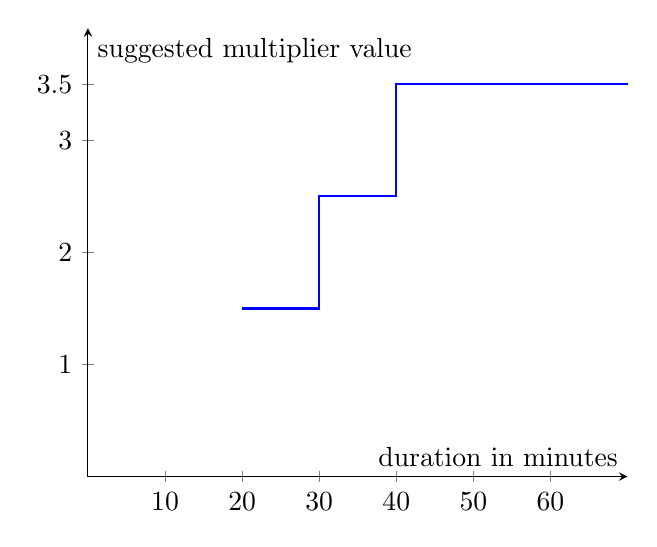
\begin{tikzpicture}
        \begin{axis}
        [
            axis lines=middle,
            xlabel={duration in minutes},
            ylabel={suggested multiplier value},
            xmin=0, xmax=70,
            ymin=0, ymax=4,
            xtick={10,20,30,40,50,60},
            ytick={0,1,2,3,3.5},
            clip=false,
            domain=20:75,
            samples=100,
        ]
            \addplot+[no marks, blue, thick, const plot] coordinates {(20,1.5) (30,2.5) (40,3.5) (70,3.5)};
        \end{axis}
    \end{tikzpicture}
\end{center}

Another more compact way to implement this is using a single rule with a more sophisticated multiplier expression.
Formula \ref{eq:bounded-linear-multiplier-function} is a valid choice for a multiplier function.

\begin{equation}
    \label{eq:bounded-linear-multiplier-function}
    f: \left[20, \infty\right) \rightarrow \left[ 1, \infty \right) : d \mapsto \min\left( 3.5, \frac{5}{40} d - \frac{3}{2} \right)
\end{equation}

Listing \ref{lst:multiplier-justification-function-linear} illustrates a rule that implements this multiplier function.
Note that the \code{condition} assures that the rule only applies to treatments with a provided laryngoscopy that took at least \code{20} minutes.
This sets the domain of the function to $\left[20, \infty\right)$.
This way, the \code{multiplier} block can safely assume that the duration is greater or equal to 20.

\lstinputlisting[
    language=json,
    style=json,
    caption={Bounded linear multiplier function},
    label={lst:multiplier-justification-function-linear}
]{code/rules/specification/multiplier-expression-linear.json}


\begin{center}
    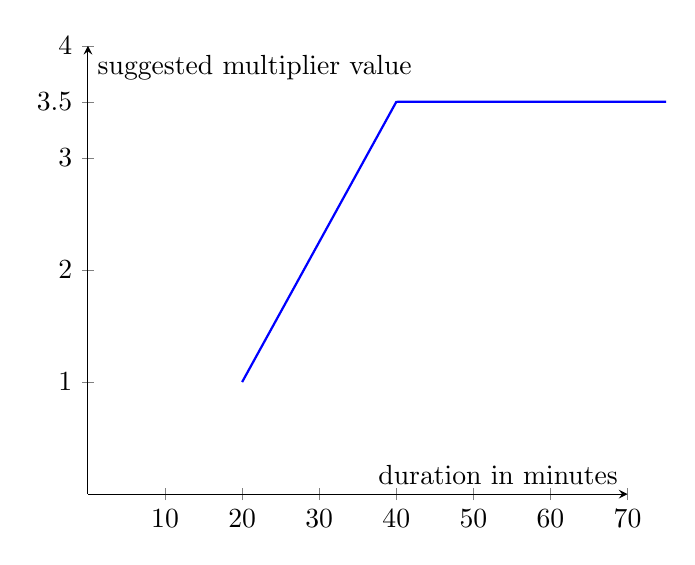
\begin{tikzpicture}
        \begin{axis}
        [
            axis lines=middle,
            xlabel={duration in minutes},
            ylabel={suggested multiplier value},
            xmin=0, xmax=70,
            ymin=0, ymax=4,
            xtick={0,10,20,30,40,50,60,70},
            ytick={0,1,2,3,3.5,4},
            clip=false,
            domain=20:75,
            samples=100,
        ]
            \addplot+[no marks, blue, thick] {min(5/40*x - 1.5, 3.5)};
        \end{axis}
        \label{plot:linear-mul-just}
    \end{tikzpicture}
\end{center}

Plot \ref{plot:linear-mul-just} illustrates the graph for the multiplier function.
The multiplier justification rule does not match ordinary laryngoscopies that take less than 20 minutes.
Note that the suggested multiplier linearly increases between 20 and 40 minutes with increasing laryngoscopy duration.
For doubtful cases where complications are so severe that the laryngoscopy takes more than 40 minutes, the rule suggests a maximum multiplier value of 3.5.
